\documentclass[12pt,a4paper]{report}
\usepackage{graphicx}
\begin{document}
\begin{titlepage}
  \centering
  
\includegraphics[scale=0.45]{Emblem72.jpg}\par
  {\scshape\LARGE National Taiwan University \par}
  \vspace{1cm}
  {\scshape\Large Term end project\par}
  \vspace{1.5cm}
  {\huge\bfseries Funtionally Reduced AIG\par}
  \vspace{2cm}
  {\Large\itshape B06705023\par Ting-Hsiang, Chiu}
  \vfill
  supervised by\par
  \textbf{Professor }Chung-Yang, Huang

  \vfill

% Bottom of the page
  {\large \today\par}
\end{titlepage}


\begin{section}{Data Structure used and architechture}
In this project, the design of data structure and data abstraction is demonstrated in the following graph.
\begin{figure}[h!]
  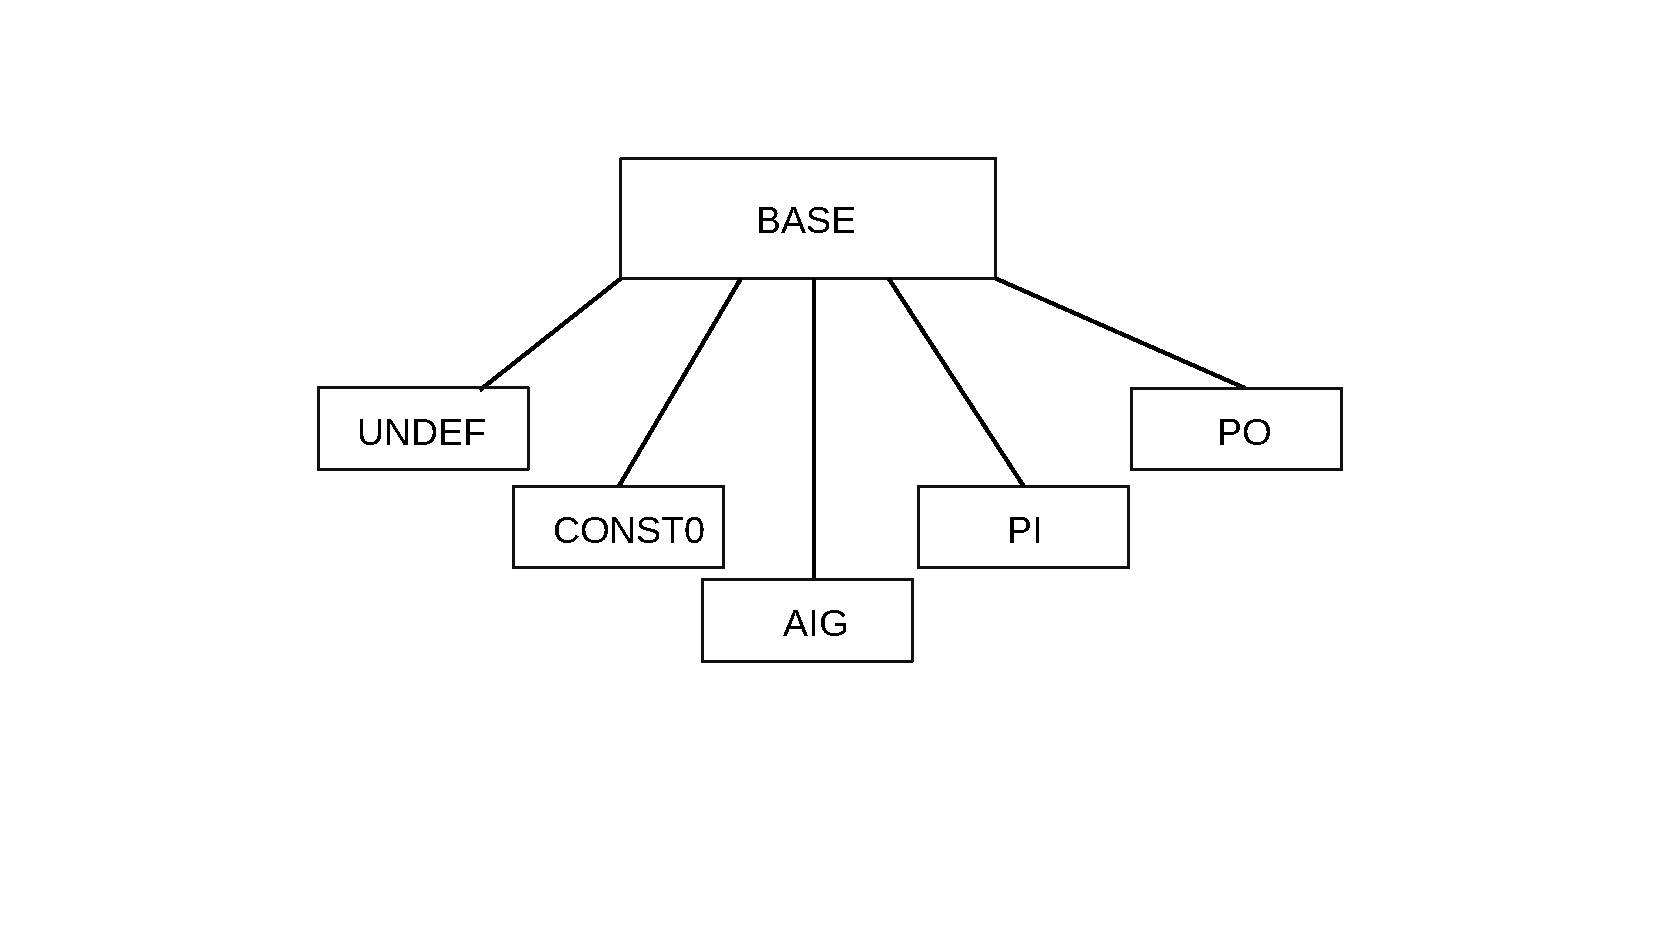
\includegraphics[scale=0.55,trim={1cm 3cm 0 10px} ]{architect.pdf}
  \caption{Structure of My fraig}
\end{figure}\\
Having a base class $base$, it stores the most common features of all gates. The member of $base$ includes:
\begin{itemize}
  \item $sizet$ ID $\rightarrow$ like the name suggests.
  \item $MultiMap$ output $\rightarrow$ Since a gate can fanin to at most two identical gates, I use multimap instead of map.
  \begin{itemize}
    \item We cannot achieve a constant time insertion, deletion, and look-up, comparing 
    to a vector based container.
    \item The benefit of multimap container is that duplicate checking is 
    in $\mathcal{O}(log(n))$ rather than $\mathcal{O}(n)$.
    \item Map container itself can handle duplicate checking, we don't need to explicitly take care of it.
    \item Fanouts of the gate is sorted comparing to vector based container.
  \end{itemize} 
  \item $float$ fanin1, fanin2 $\rightarrow$ If the gate gets an inverted fanin, fanin will become negative.
  \begin{itemize}
    \item Due to the non-exist of $-0$, I will add $0.1$ before negating the number.
    \item 2 float together occupies 8 byte in total. 
    \item In comparison, if we store location and inverse seperately, it will occupy up to 16 byte.
  \end{itemize}
  
  \item $int$ line $\rightarrow$ which line it is declared in the aag file.
  \item $int$ printidx $\rightarrow$ used with global variable, $printidxs$.
\end{itemize}
Apart from those common features in $base$, there are still some minor differences in each
inherited class. Such as,
\begin{itemize}
  \item SymbolicName $\rightarrow$ PI and PO
  \item inSig $\rightarrow$ PI
  \item outSig $\rightarrow$ PO
  \item Sig1,Sig2 $\rightarrow$ for AIG
\end{itemize}
The reason why CONST0 and UNDEF exist is because I want to avoid accessing nullptr in $gates$.\\
These two classes are purely served as a identifying null pointer and UNDEF.
\end{section}
\begin{section} {Structure of CirMgr}
\begin{itemize}
  \item vector PO $\rightarrow$ Polymorphic based container.
    \begin{itemize}
      \item Stores all the POs.
    \end{itemize}
  \item vector gate $\rightarrow$ Polymorphic based container.
  \begin{itemize}
    \item  Stores all the gates except PO.
  \end{itemize}
  \item array POnum $\rightarrow$ Value appeared in aag file's output section.
  \item array PInum $\rightarrow$ Value appeared in aag file's input section.
  \item HashSet myKey $\rightarrow$ Used in Strash.
  \item HashSet myFECgrps $\rightarrow$ Used in Sim.
\end{itemize}
\end{section}
\begin{section}{Rnadom aag Generator}
  This came from HW6, when I initially doubted the usefulness of this program. Later turn out to be a 
  really great helper in testing out my design.

  To really test out all the case and correctness of my program, I build up a Directed Acyclic Graph 
  generator. It takes several number as parameter to build up the graph, including PI, PO, amount of aags

  Generating an aag file with more than 200,000 gates, just took less than a second.
  Thanks to Random Number generator, it can create lots of unused, undefined, unreachable gates,
  by simply modifying the value of $\frac{PI}{PO}$. In normal cases, when I want to test out 
  the correctness of my program, I usually set it to $1$ or $1.2$. For extreme cases, when I want 
  to stress out the algorithm, the value goes beyond 0.01, and have aags more than 100,000.

  If you think this is an useful design or may be helpful to students taking this class in the future, 
  please do let me know. I can make this part of the source code become an
  independent Web page on Github.(Just like
  aag-visualizer)
\end{section}
\begin{section}{Sweep}

  Originally, I plan to keep a DFS list for ease of tracking "Reachable" gates. However,
  I came to find out that the job can be done by traversing the graph. Also, keeping the DFS list
  means I have to update it whenever I have modifications to the aig graph. Or, I have to
  update it after modifying the graph. In contrast, traversing and sweeping at the same time just seems to make sense.
  Because when we finish traversing, we won't step into any other sweeped gates, and no other operations or 
  things need to take care of after traversal.\\
  For each gate that I want to sweep out, the following process needs to be taken:
  \begin{itemize}
    \item Remove the gate from the fanout of its fanin.
    \item Set the fanin of the fanout of the gate to null.
    \item delete the gate from all gate, set it to $null$ pointer.
  \end{itemize}

  {\textbf{Complexity: }$\mathcal{O}(|E|)$} There is no clear definition of $E$ here, so I define
  it to be the links between two gates.\\
  
  Even if we did try to visit only those gates not in the DFS list, we still have a complexity of $\omega(n)$

\begin{subsection}{Performance and Bottleneck}
  Some minor cnostant speed improval can be implemented such as, saving the DFS list rather than 
  traversing the whole graph again. This may save some time when the DFS tree only occupies a 
  small portion of the graph.

  If we taken space complexity into consideration, which is kind of rare these days, my code use 2 times
  more than the ref code used, resulting in around 40 mb.
\end{subsection}
\begin{subsection}{Comparisons}
  In the testing process, I only focus on graphs that has aig gates more than 100,000. Under this
  circumstance, a minor inefficient in each step can sum up to be a true disaster.\\

\textbf{Performance: } I designed two extreme cases, one is a graph with only 1 output and 20000 PI, 120,000 aig gates.
The other one is inversing PI and PO,(1 PI, 20000 PO). The first case my code is just running as fast as ref code did.
To be strict enough, they have difference less than 0.5 second. In actual running time, both of them
runs less than a second.


\end{subsection}
\end{section}
\begin{section}{Strash}
  Same as previously mentioned, I traverse the graph and put the fanin pair and index into HashSet. Whenever a
  collision occurred, meaning that there is a structually equivalent gate existing. I will then remove
  that latter gate.

  I introduced HashSet in HW7 to help us out from using $STL$'s unordered map. Also, we need to define
  out own data structure to store the pair of inputs and the index. The structure is as follows:
  \begin{itemize}
    \item integer $ID$
    \item pair of integers $(input1,input2)$
    \item operator() $\rightarrow$ generate hash value
    \item operator== $\rightarrow$ used as comparison in the hashset.
  \end{itemize}
  \begin{subsection}{Performance}
    To generate a graph rich in "strashable" aig gates, is really hard. I have to change the rules of 
    building up the DAG, because it is choosing randomly without any restrictions(it still considers
    the DFS ordering). Now I have to store those pairs of fanins, and randomly insert them into some 
    of the aig gates. \\
    Same as previous, I have to build up a graph that is rather tall instead of fat
    and wide. The point to really stress out the performance is to build up two identical graph and then
    merging(reducing) them into one.\\

    \textbf{Performance:} The best case, which is a very normal graph, performs as well as the ref code did.
    The worst case, which I designed specifically, performs slightly slower than the ref code.
  \end{subsection}
\end{section}

\begin{section}{Optimize}
  As mentioned in \textbf{0.3}, I trverse the aag graph instead of visiting the DFS list.

  Initially, I came up with two approach of optimizing the whole circuit. One is to optimize the 
  circuit wihout caring the DFS order. That is, optimizing from $gate[0]$ up to $gate[m]$. However,
  I later discover that it cannot be proven to be correct. For example, if we optimize gate $A$ first,
  then $B$, $C$. Not following the hierarchical ordering (DFS number), may result in failing to merge
  or identify a gate with non-CONST input as a CONST0 or CONST1 output. Now, this, brings us to the second
  method

  If we follow by the hierarchical order, a bottom-up manner, we can avoid the pit-fall 
  mentioned above. 

  Taking one step forward, let's look at what can happen to each gate. First up, a gate can have the
  following input pattern.
\begin{itemize}
  \item Identical Input
  \begin{itemize}
    \item Erase the gate from fanout of their fanins.
    \item Erase the gate from fanin of their fanouts.
    \item Set the fanin of fanout of the gate to CONST1.
    \item Add fanout of the gate into fanout of CONST 1.
  \end{itemize}
  \item Inversed Input
  \begin{itemize}
    \item Erase the gate from fanout of their fanins.
    \item Erase the gate from fanin of their fanouts.
    \item Set the fanin of fanout of the gate to CONST0.
    \item Add fanout of the gate into fanout of CONST 0.
  \end{itemize}
  \item A CONST0 input regardless of the other fanin
  \begin{itemize}
    \item Erase the gate from fanout of their fanins.
    \item Erase the gate from fanin of their fanouts.
    \item Set the fanin of fanout of the gate to the non-CONST1 gate.
    \item Add the fanout of the gate to CONST0.
  \end{itemize}
  \item A CONST1 input regardless of the other fanin
  \begin{itemize}
    \item Erase the gate from fanout of their fanins.
    \item Erase the gate from fanin of their fanouts.
    \item Set the fanin of fanout of the gate to the non-CONST1 gate. 
    \item Add the fanout of the gate to fanout of fanin of the gate
  \end{itemize}
\end{itemize}
\begin{subsection}{Performance and Bottleneck}
  \textbf{Performance: } Not much difference as the ref code performs. However, there is still some part
  worth mentioning. I can improve my code by changing some of these parts.
  \begin{itemize}
    \item Output
    \begin{itemize}
      \item I am currently using a multimap for storing outputs, it cannot achieve a $\mathcal{O}(1)$ insertion
      \item If I can utilize HashMap, it can slightly improve from $\mathcal{O}(log(n))$ to $\mathcal{O}(1)$.
    \end{itemize}
    \item direct access
    \begin{itemize}
      \item This is kind of a trade-off between efficiency and fail-safe. I designed lots of helper function
            to protect and acquire objects.
      \item The cost is to build up a somehow big function overhead. Draggin the processing speed down to
      a notifiable level.
    \end{itemize}
  \end{itemize}
\end{subsection}
\end{section}
\begin{section}{Simulation}
  Firstly, because the simulation needs to be done by some kind of topological ordering up to PO,
  we have to simulate from bottom-up. 
  Only sending signal to those that can be reached from POs, otherwise it is meaningless. For every gate that
  is possible to send out signal (PI,PO,AIG,CONST0), I have a virtual function defined in base class called $genResult()$. This allows me to
  handle gates seperately, concerning their input(s). With this in hand, we can start to send out signals.\\
  For each pattern I want to send into a specific PI, I store that signal, either 0 or 1, inside a bit.
  Every 64 patterns sent into that PI can be packed into a $size$ $t$ data type.\\
  To be hoest, I really think it is a great discovery of parallel pattern. It goes through 64 pattern in one run, which
  can tremendously save time when we have say 10 million patterns. Apart from that, the function overhead or
  resource occupied for 64 patterns is nearly none and can be done at worst in constant time.\\
  After inserting those signals in PI, we can then fire up the simulation process. Same as previous
  mentioned, we start off the process by DFS, untill we reach the bottom-most AIG gate.\\
  After that, we traverse backward and conduct the post-work. In this case, post work will be
  to set two of your fanins' $genResult$ as your fanin. Then, repeating this process until we reach PO,
  we would have done a PO's simulation.
\begin{subsection}{Performance and Bottleneck}
  \textbf{Performance:} Gladly enough to say, comparing my result with teachers. I simulated $sim13$ with pattern 13. It turns out that we are
  having the same performance. However, if I self generate an input of 20,000 pattern, it is having a bit differnce comparing
  to ref code. In actual running time, I am almost three times as slow as teachers code ran.
  
  \textbf{Bottleneck:} The bottleneck I cannot break through here is that I will traverse the aag graph again and again.(Every 
  64 patterns simulated) Whereas,
  ref code is only sending the signal through the DFS tree(or DFS list). Though, it is only a minor difference in one run(one pattern).
  This will be a huge problem if the patterns soar. Say 1,000,000 patterns, and each pattern I am 10$m$s behind, then my code
  will run have to run an extra 3 hours to complete the simulation.
\end{subsection}
\end{section}
\begin{section}{My Opinion}
  As Ric had said in class, ideally I should have finish $Sim$ before term-end. Otherwise, there will
  be not much time left to carry out the whole project. It is a pity that this class I should have spend
  a little more time on finishing the Final Project. It is not until this class do I understand the 
  importance, ignorance of myself, and lack of professional coding background. I cannot emphasize more
  of how I appreciate Ric has brought about to this class and the intensity he had created for the 
  7 homeworks. The class not only sooth the desire of writing lots of lots of code, but also told me
  how to write as less code and be as algorithmically efficient as possible.\\
  As a student not majoring in EE/CS but in IM, I think maybe the final project can become a team project.
  With some restrictions like, students did well in previous homeworks must group up with not so professional
  ones. As Ric had mentioned so many times in class, software development pattern, github, co-working and code review...etc.,
  I think having a final "team" project can help us practice more on those skills.\\
  Also, why can't we submit our works via github?\\
  \\\\\\\\\\
  It Has Really Been An \textbf{INTENSE} class. Respect to Ric and all the TAs involved.
\end{section}
\begin{section}{Contact Information}
  \begin{itemize}
    \item Email: b06705023@ntu.edu.tw, alternative: louiechiu@gmail.com
    \item Mobile: +886-938-715-869
  \end{itemize}
  \end{section}

\end{document}
